% !TEX TS-program = pdflatex
% !TEX encoding = UTF-8 Unicode

%************************************************
\chapter{Sistema di diffusione}
\label{chp:Sistema di diffusione}
%************************************************

\epigraph{Come un rosone nel cuore di un tempio immenso}{\textit{Antonin Artaud}}

La diffusione sonora di Vitres de Son è basata sull'utilizzo di 9 dei 22 altoparlanti presenti nella cupola sonora "Il suono di Piero" costruita nel all'interno dell'Aula I del III piano del conservatorio Santa Cecilia, in Roma. Sfruttare solo una parte della cupola è legato alla composizione, sia a livello di figura nella quale far adagiare l'esecutore e l'oggetto sonoro, sia a livello di diffusione. Il rosone del sottotitolo sta ad indicare, appunto, la disposizione delle casse. Come nella figura sopra, notiamo che le casse disposte a triangolo, sono i vertici di un arco, significante dell'immagine del rosone. Il suono confluisce al centro e la microfonazione puntuale, ci dà la possibilità di seguire il suono nei suoi spostamenti.

Tendo a sottolineare che la spazializzazione del suono è data esclusivamente dalla microfonazione.
<<<<<<< HEAD
Per la costruzione del sistema di diffusione ho utilizzo gli scritti introduttivi che sono allegati a molte partiture di Luigi Nono (cit. Postpraeludium e Prometeo). Ovvero, il compositore non è più slegato da una realtà percettiva e teatrale del produzione sonora, ma diventa artefice della disposizione degli altoparlanti e del pubblico all'interno dell'ambiente d'ascolto. \\
=======
Per la costruzione del sistema di diffusione ho utilizzo gli scritti introduttivi che sono allegati a molte partiture di Luigi Nono (cit. postpraeludium e Prometeo). Ovvero, il compositore non è più slegato da una realtà percettiva e teatrale del produzione sonora, ma diventa artefice della disposizione degli altoparlanti e del pubblico all'interno dell'ambiente d'ascolto.

>>>>>>> 6757b0572a7e90c3d05cd9e7e841b5c76286f9f4
Vediamo nel dettaglio il sistema di ripresa e la diffusione audio che da partitura diventano parte integrante della composizione.

\section{Sistema di ripresa}
La diffusione audio avverrà tramite l'utilizzo di un sistema di diffusione omnidirezionale che renderà possibile la diffusione omogenea del materiale acustico ed elettronico prodotto da Sp.i.r.e..

\begin{itemize}
	\item{Scheda Audio 8in 9out}
	\item{4 piezoelettrici}
	\item{2 microfoni dpa omnidirezionali}
	\item{2 microfoni Cardioide}
	\item{Cablaggio}
	\item{1 Amplificatore di potenza da 4 canali a 4 Ohm}
	\item{Computer\\}
\end{itemize}

\begin{figure}[htbp]
\begin{center}
\includegraphics[width=.99\textwidth]{ripresa.jpg}
\caption{Ripresa microfonica dello Sp.I.R.E.}
\label{default}
\end{center}
\end{figure}

%\begin{center}
%\includegraphics[width=1.\textwidth]{ripresa.jpg}
%\end{center}

Strumenti utilizzati:

%\begin{center}
%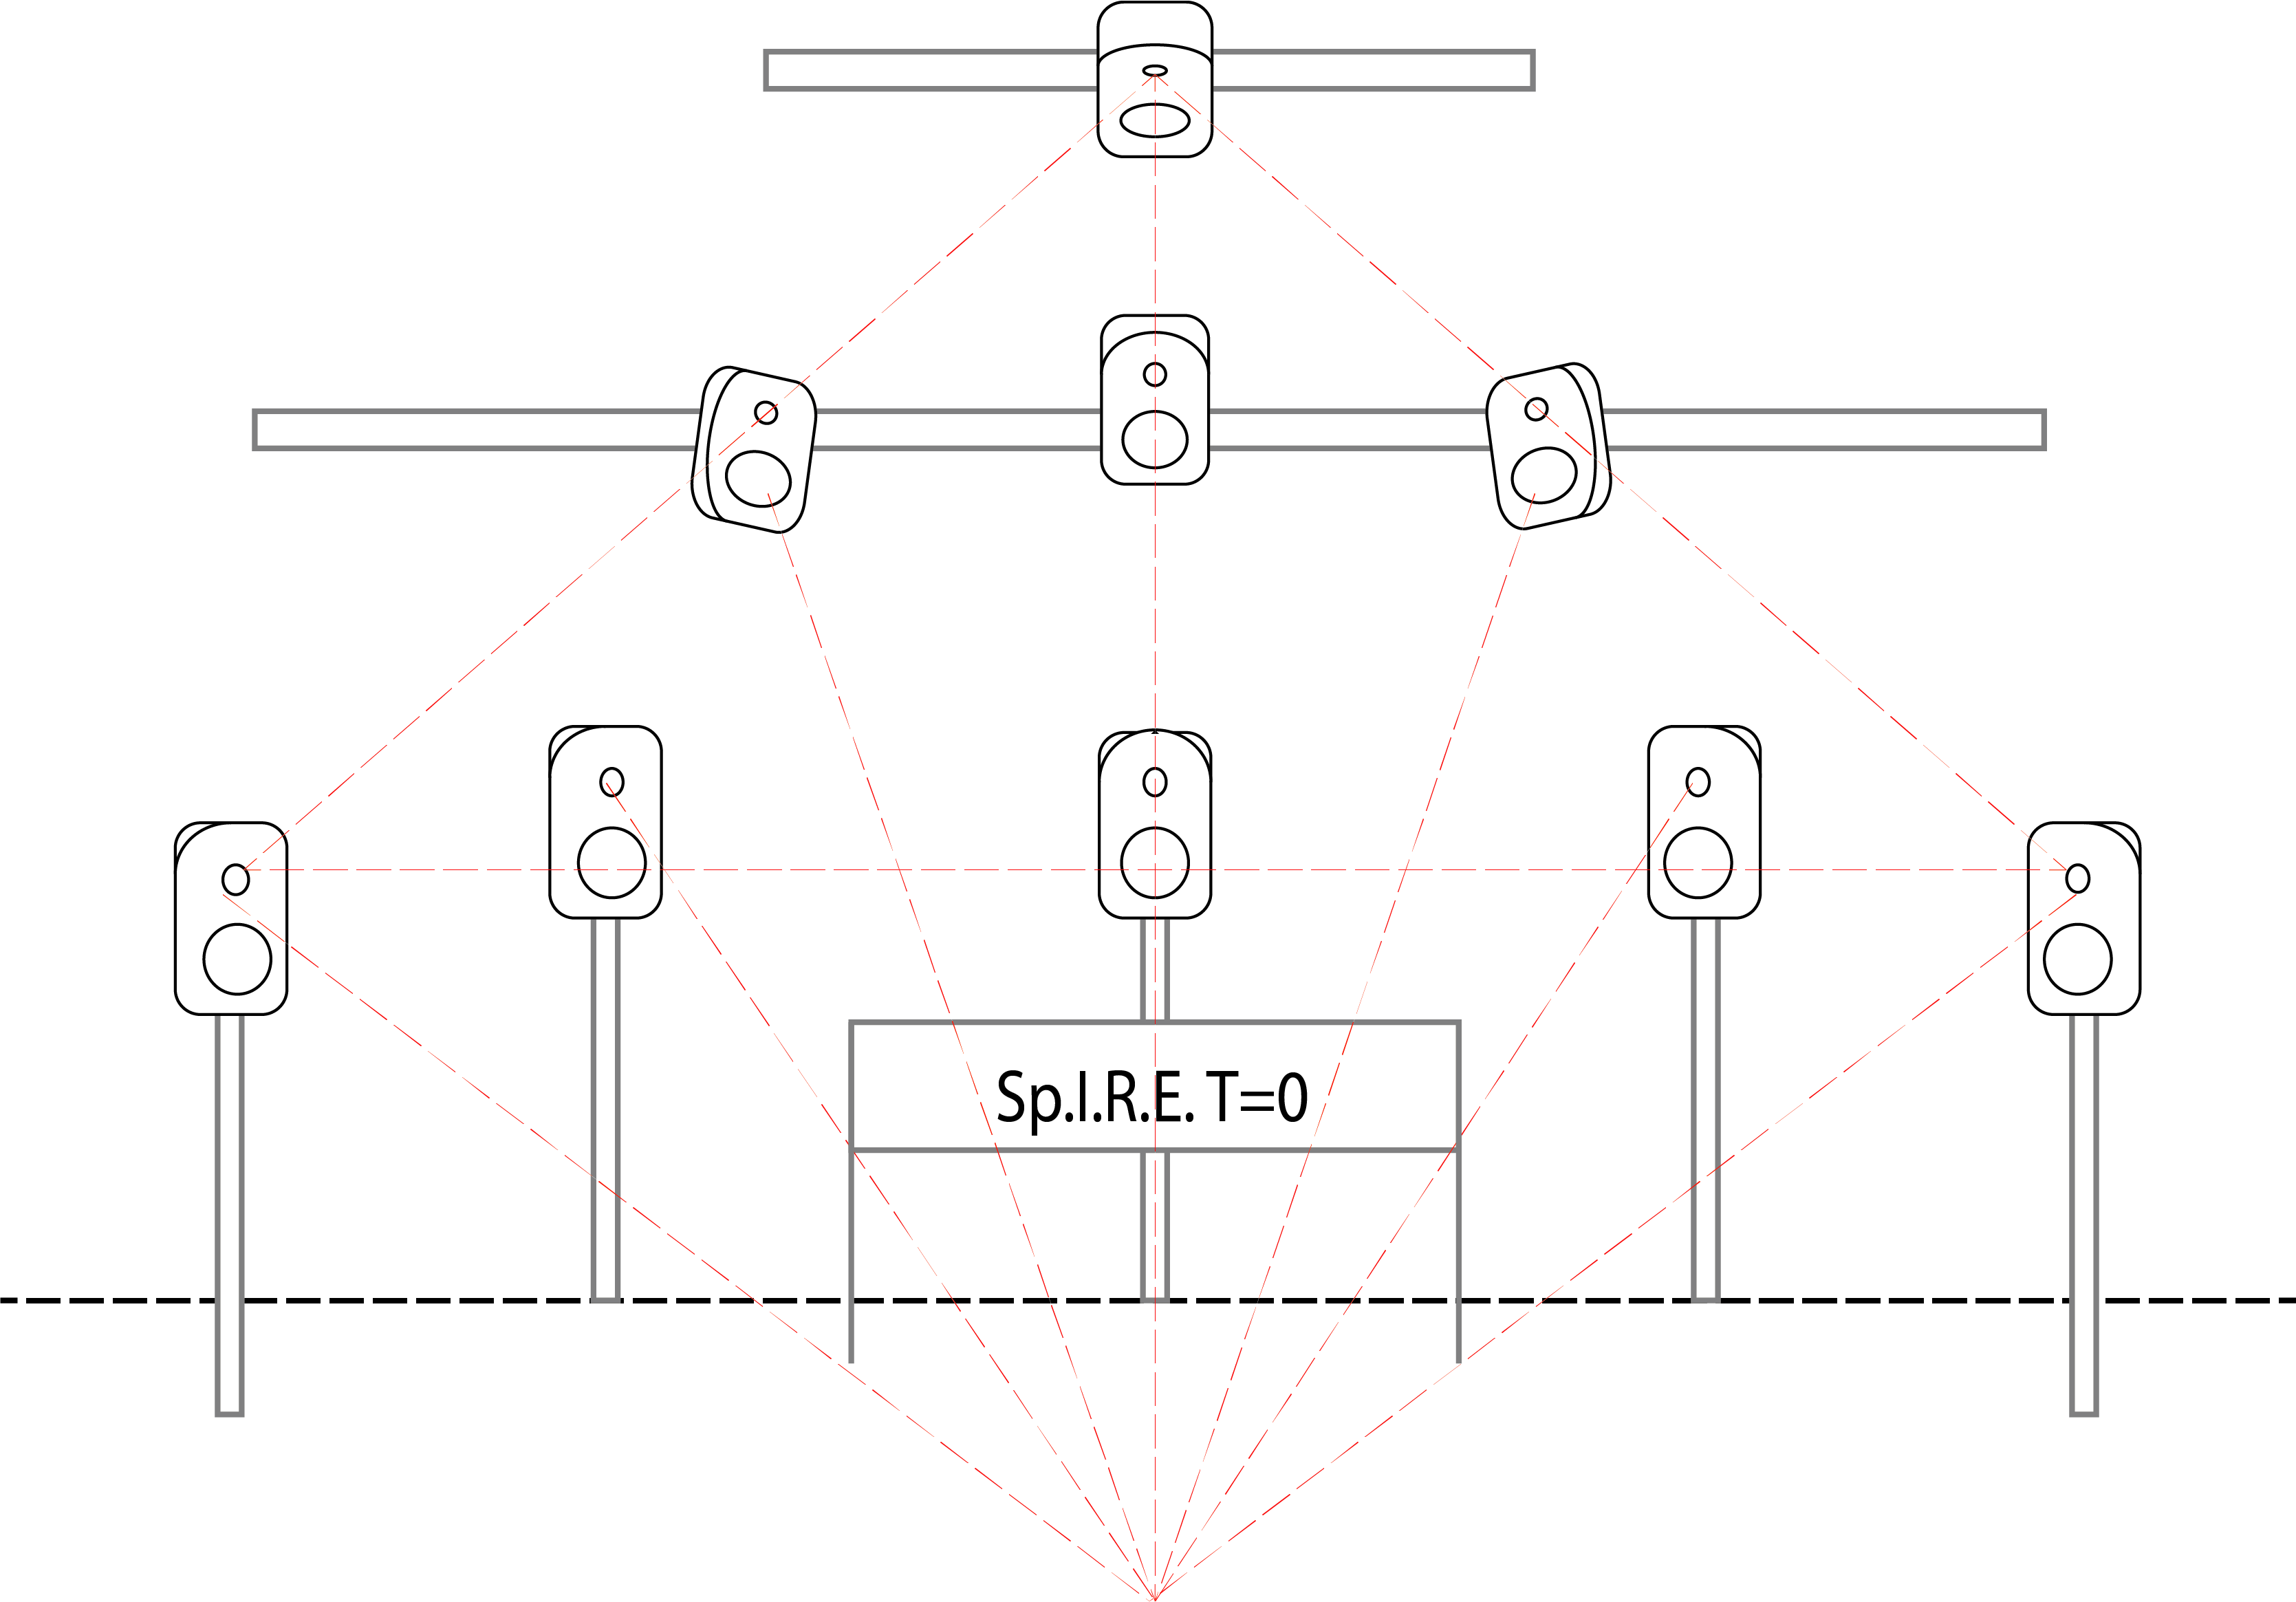
\includegraphics[width=1.\textwidth]{diffusione.png}
%\end{center}

\begin{figure}[htbp]
\begin{center}
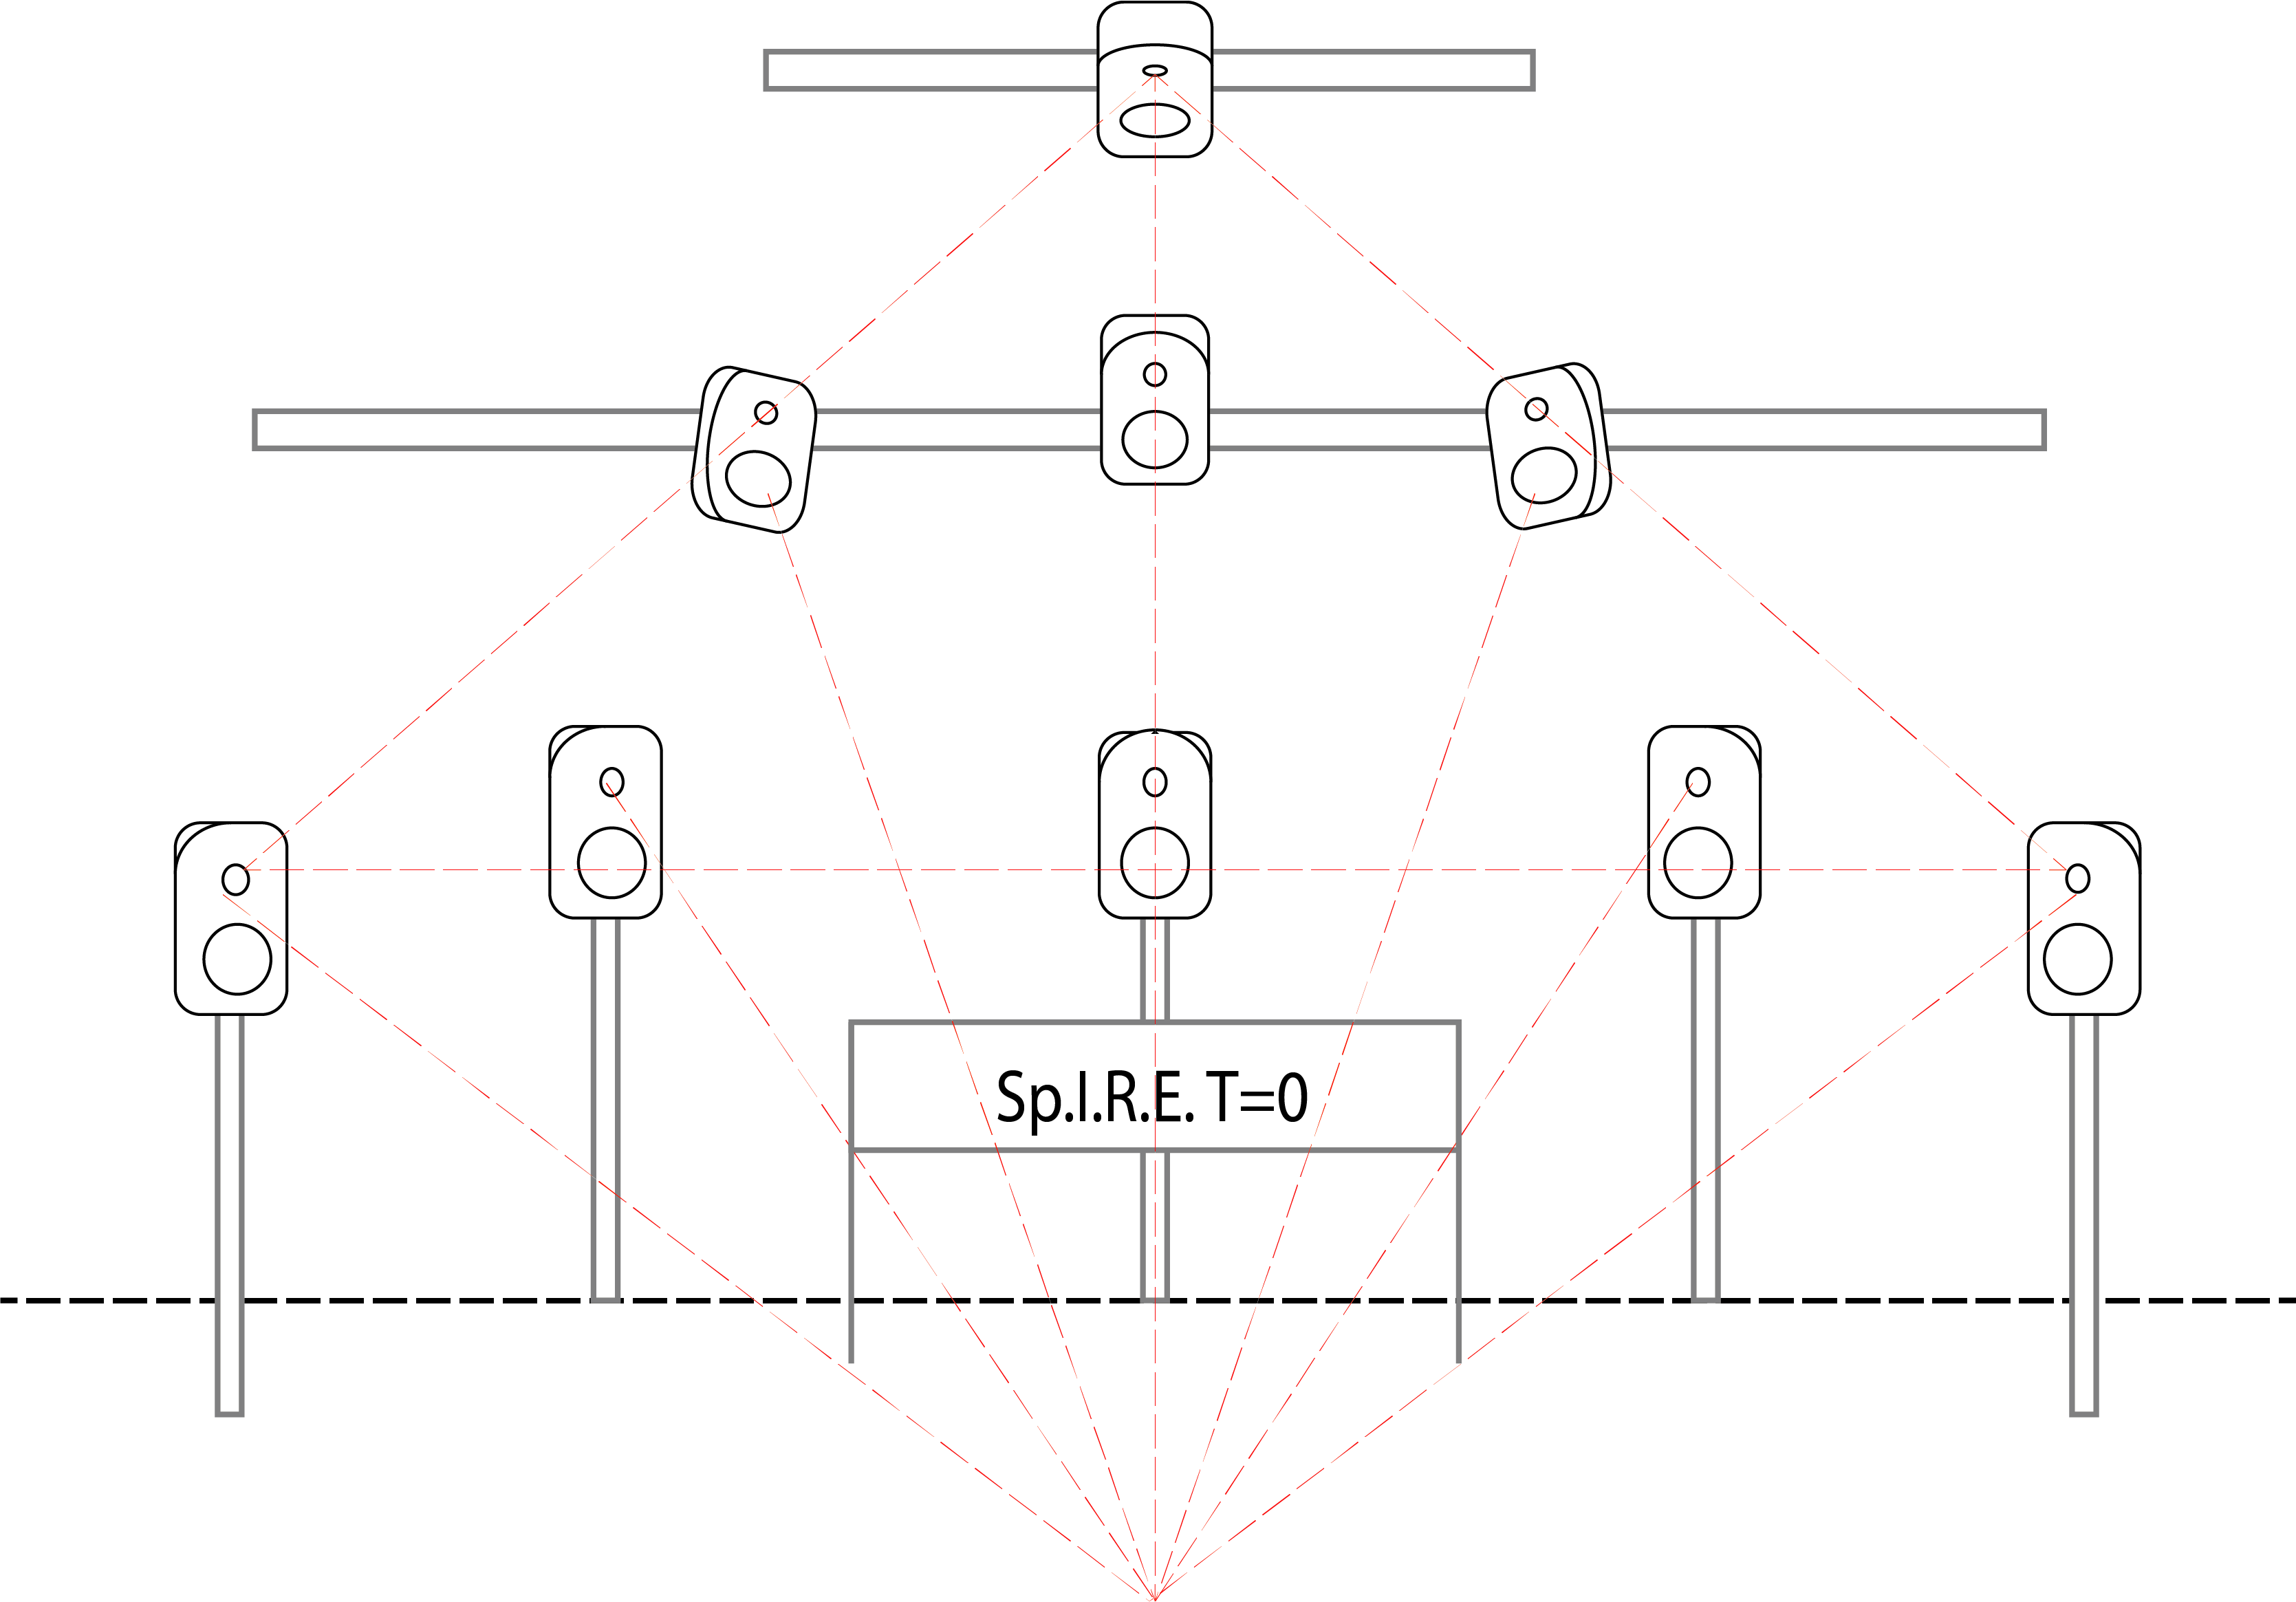
\includegraphics[width=.99\textwidth]{diffusione.png}
\caption{Diffusione a \textit{A Rosone} di Vitres de Son}
\label{default}
\end{center}
\end{figure}

\begin{itemize}
	\item{Sp.i.r.e.}
	\item{Amplificazione trasparente}
	\item{9 Altoparlanti}
\end{itemize}

\section{Diffusione} %audio e B-Format} non mi pare ci sia nulla di B-Format nel testo

\begin{figure}[htbp]
\begin{center}
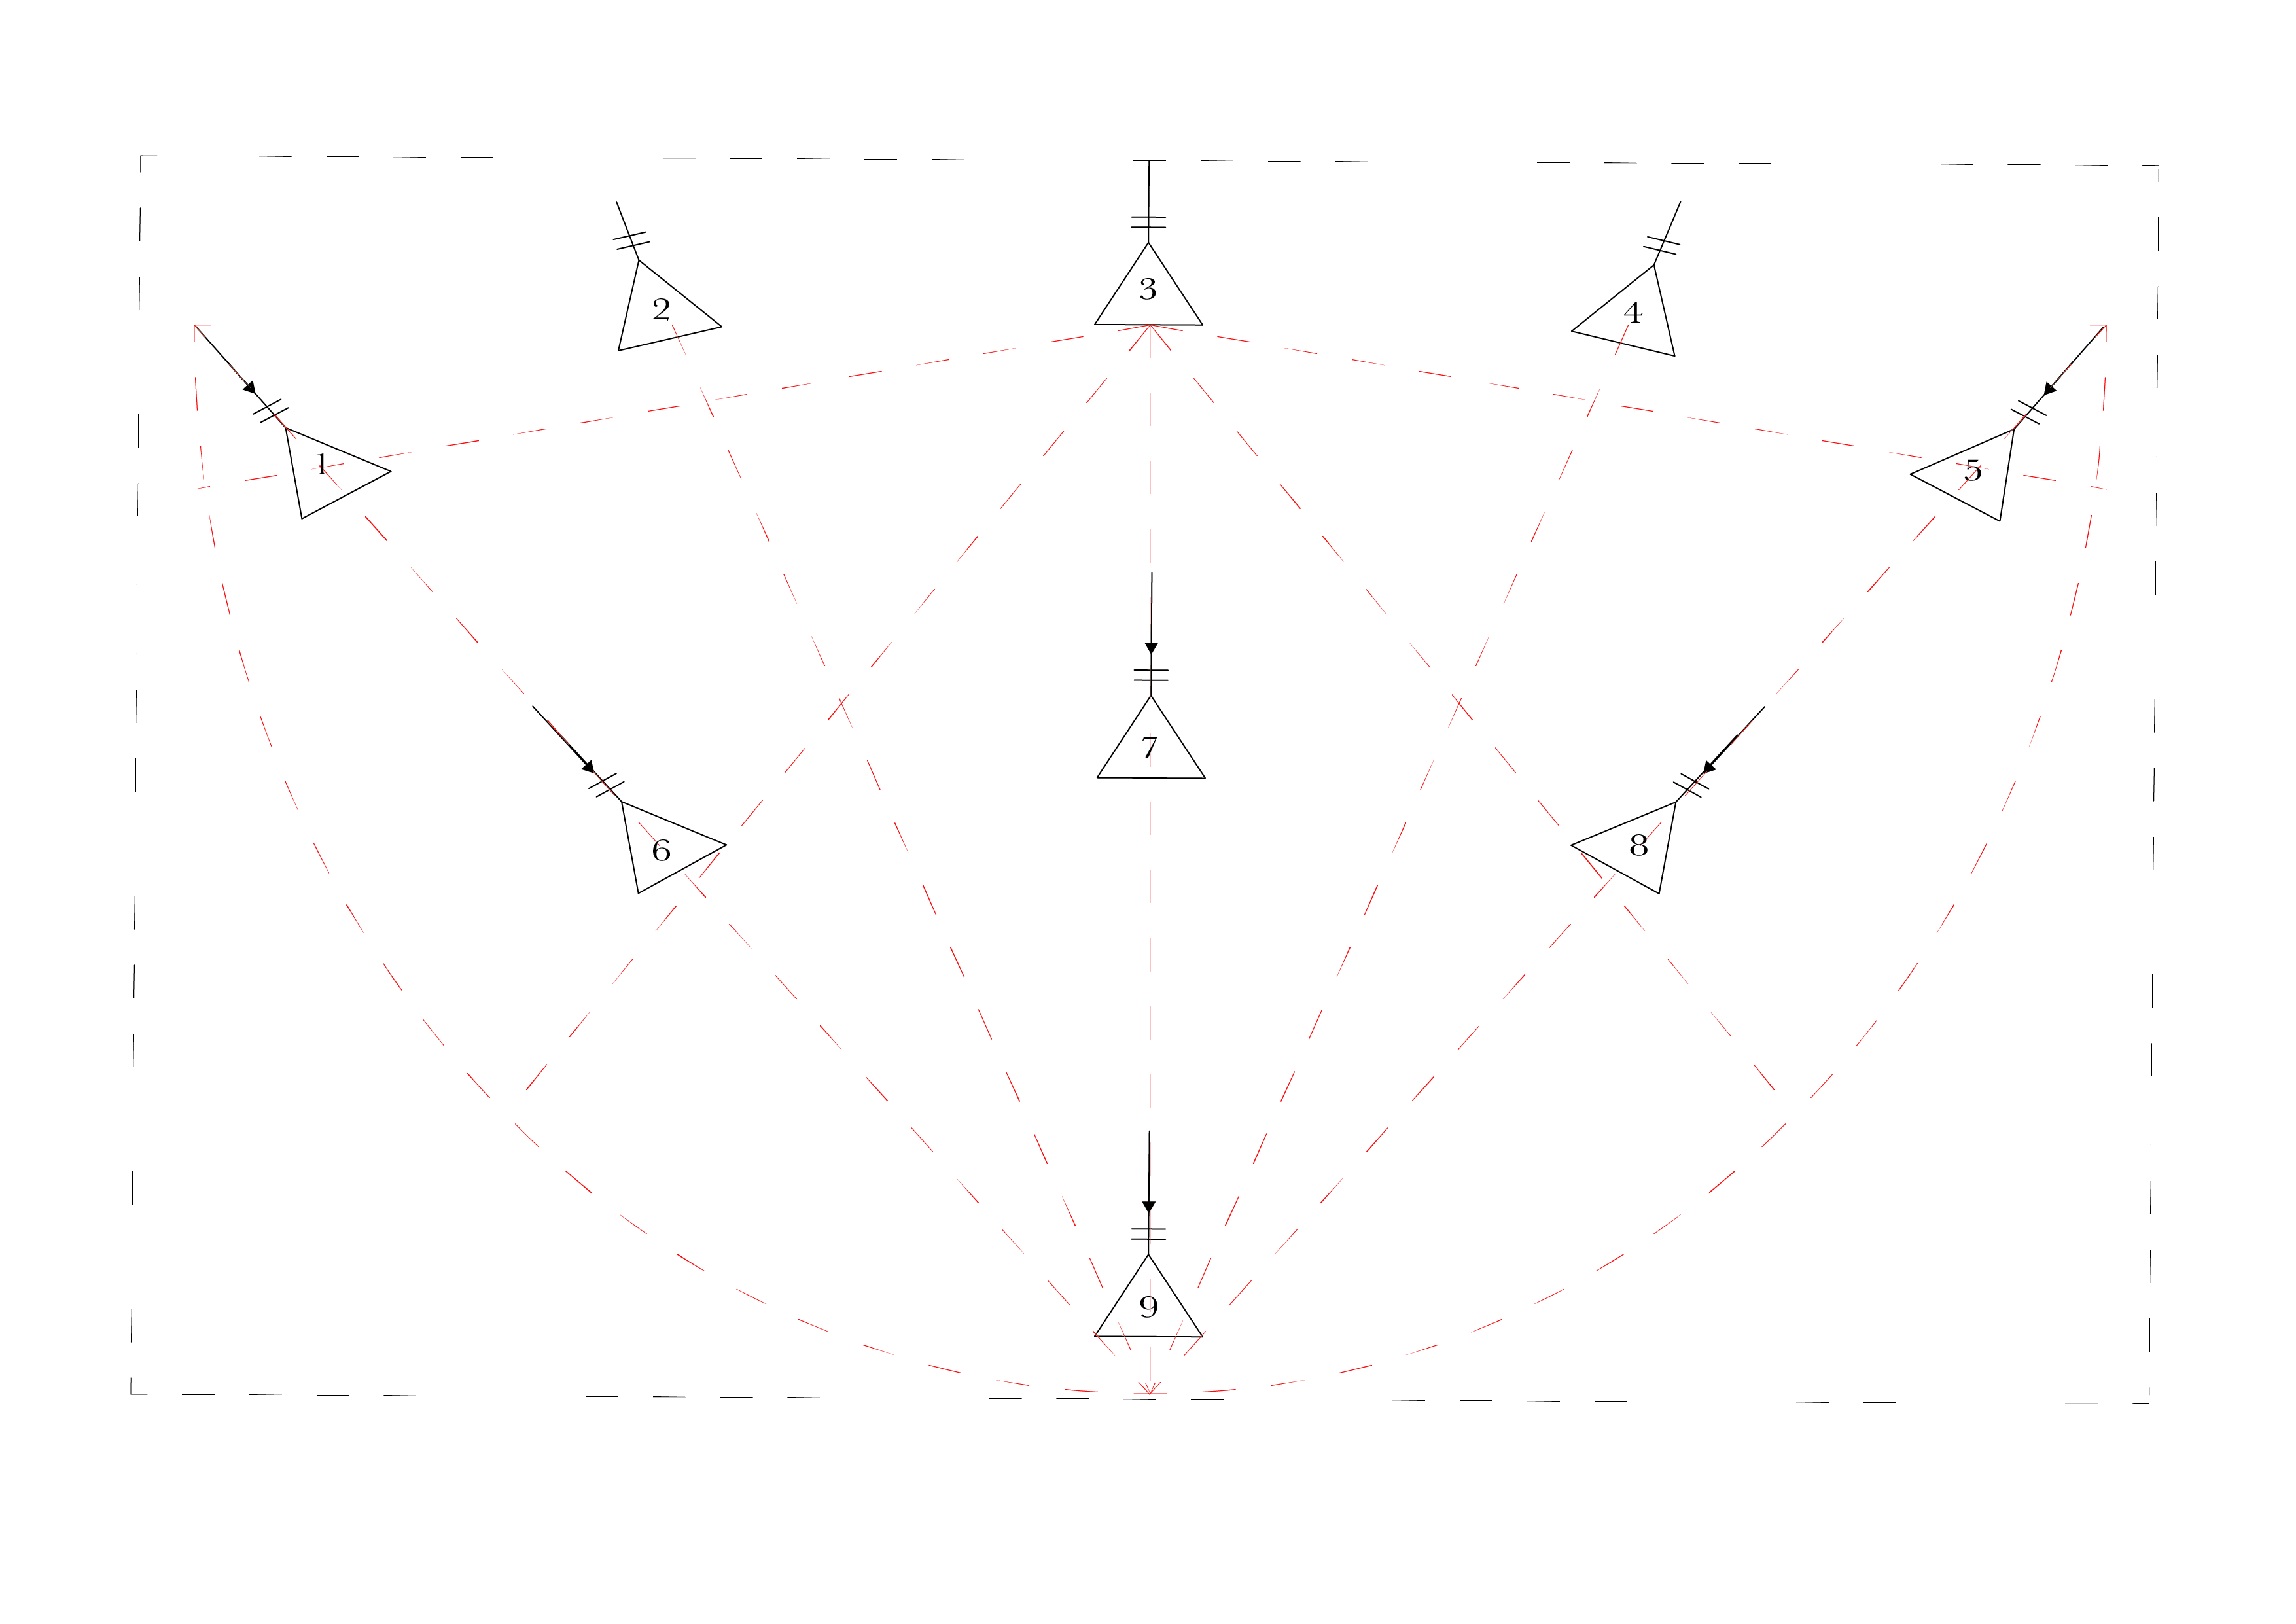
\includegraphics[width=1.2\textwidth]{legenda02.png}
\caption{Diffusione a \textit{A Rosone} di Vitres de Son}
\label{default}
\end{center}
\end{figure}

Per schematizzare e disegnare la diffusione audio, ho utilizzato come esempio gli scritti introduttivi e le legende di due partiture contemporanee. Specificatamente: Mantra di Karlheinz Stockhausen e Prometeo, Tragedia dell'ascolto di Luigi Nono. Nella partitura di Stockhausen vediamo come il compositore esplica lucidamente il rapporto che c'è tra diffusione ed elaborazione del segnale, in un solo schema racchiude sia la diffusione che l'elaborazione, un po' come la partitura di \textit{Ecosistemi} di Agostino Di Scipio.

<<<<<<< HEAD
Nono, nel Prometeo, aggiunge agli schemi degli algoritmi e di diffusione, anche la disposizione del pubblico in sala. Questa è un passo importante per la storia della musica elettroacustica, perché alla modalità d'ascolto si aggiunge un fattore importante per la stesura di un lavoro compositivo: la regia. Nono era sempre attento al rapporto fra diffusione del suono e disposizione dell'ascoltatore. \\
=======
Nono, nel Prometeo, aggiunge agli schemi algoritmici e di diffusione, anche la disposizione del pubblico in sala. Questa è un passo importante per la storia della musica elettroacustica, perché alla modalità d'ascolto si aggiunge un fattore importante per la stesura di un lavoro compositivo: la regia. Nono era sempre attento al rapporto fra diffusione del suono e disposizione dell'ascoltatore.

>>>>>>> 6757b0572a7e90c3d05cd9e7e841b5c76286f9f4
Prendendo ad esempio i maestri, ho lavorato su un'irradiazione tale da poter favorire un spostamento del suono a livello spaziale. La tipologia di microfonazione e la disposizione dei diffusori, permette:

\begin{itemize}
\item{La disposizione dei microfoni (figura 19) rende possibile un movimento spaziale del segnale. Sicuramente anche la scrittura ho tenuto conto di questo effetto, scrivendo gesti puntuali quando ritenevo strutturale uno spostamento della fonte sonora nello spazio.}
\item{La serie di filtri presente a valle, prima della diffusione, permette un movimento del suono verso l'alto, dato anche dall'utilizzo di diffusori sospesi al di sopra dello strumento}
\end{itemize}

L'amplificazione trasparente ed il filtraggio danno corporeità al suono e oltre a rendere possibile una spazializzazione realistica dello strumento, si da anche la possibilità alla stanza di risuonare su determinate frequenze dato il lungo decadimento dello Sp.I.R.E..
